\documentclass[a4paper,11pt]{article}

% --- ENCODING & LANGUAGE ---
\usepackage[english]{babel}
\usepackage[T1]{fontenc}
\usepackage[utf8]{inputenc}

% --- GEOMETRY ---
\usepackage[margin=2.5cm]{geometry}
\setlength{\parindent}{0pt}
\setlength{\parskip}{0.8em}

% --- GRAPHICS, MATH, TABLES ---
\usepackage{graphicx}
\usepackage{float}
\usepackage{subcaption}
\usepackage{amsmath, amssymb}
\usepackage{siunitx}
\usepackage{booktabs}
\usepackage{xcolor}
\usepackage{listings}
\usepackage{fancyhdr}
\usepackage{hyperref}
\hypersetup{colorlinks=true, linkcolor=black, urlcolor=blue, citecolor=black,
            pdftitle={Practice 3: Equation of State of a Lennard-Jones Fluid}}
\usepackage[capitalise]{cleveref}

% --- HEADER (same as previous practices) ---
\pagestyle{fancy}
\fancyhf{}
\lhead{
\includegraphics[height=1cm]{images/upc.png}}
\rhead{
\includegraphics[height=1cm]{images/ef.png}}
\cfoot{\thepage}
\renewcommand{\headrulewidth}{0.4pt}
\setlength{\headheight}{40pt}

% --- SECTION TITLES: "Exercise N" without numbers ---
\newcommand{\exercise}[1]{\section*{Exercise #1}\addcontentsline{toc}{section}{Exercise #1}}
\newcommand{\statement}[1]{\textbf{#1}\par}

% --- CODE STYLE ---
\definecolor{codebg}{rgb}{0.96,0.96,0.96}
\definecolor{codekw}{rgb}{0.10,0.20,0.85}
\definecolor{codetype}{rgb}{0.20,0.55,0.70}
\definecolor{codestr}{rgb}{0.75,0.10,0.10}
\definecolor{codecom}{rgb}{0.10,0.55,0.10}
\definecolor{termbg}{rgb}{0.15,0.15,0.15}

\lstdefinestyle{fortran}{
  language={[95]Fortran},
  backgroundcolor=\color{codebg},
  basicstyle=\ttfamily\scriptsize,
  keywordstyle=\color{codekw},
  commentstyle=\color{codecom},
  stringstyle=\color{codestr},
  morekeywords={real,integer,logical,character,allocatable,parameter,intent,kind,anint,floor,inquire,cycle},
  numbers=left, numberstyle=\tiny\color{gray}, numbersep=10pt,
  frame=lines, rulecolor=\color{gray!40},
  breaklines=true, showstringspaces=false, tabsize=4,
  xleftmargin=1.5em, framexleftmargin=0.5em
}
\lstdefinestyle{python}{
  style=fortran, language=Python,
  morekeywords={True,False,None}
}
\lstdefinestyle{terminal}{
  backgroundcolor=\color{termbg},
  basicstyle=\ttfamily\scriptsize\color{white},
  frame=lines, rulecolor=\color{black},
  numbers=none, breaklines=true, showstringspaces=false,
  xleftmargin=0pt, framexleftmargin=0pt
}

\begin{document}

% ================= COVER =================
\pagenumbering{gobble}
\thispagestyle{empty}

\begin{center}
\vspace*{2.5cm}

\includegraphics[width=3.5cm]{images/upc.png}\\[2.5cm]

{\large\textbf{Physics Engineering}}\\[0.4cm]
{\Large\textbf{Computer Simulation of Condensed Matter}}

\vspace{2.5cm}
\hrule
\vspace{6mm}
{\huge\bfseries Practice 3: Equation of State of a Lennard-Jones Fluid\par}
\vspace{6mm}
\hrule
\vspace{8mm}

{\large\textbf{Víctor Sender, Leo Vidal}}\\[2mm]
{\large\textbf{20 November, 2026}}
\end{center}

\newpage
\pagenumbering{arabic}
\setcounter{page}{1}

% ================= EXERCISE 1 =================
\exercise{1}
\statement{Write a MC code for a $(N,V,T)$ simulation of a Lennard-Jones system. You can use the
\texttt{leapfroglj.f} program as the starting point.}

The code (\texttt{mcnvt.f90}, \hyperref[app:code]{Appendix A}) is built from the leapfrog program of Practice 2 by
removing everything related to velocities and forces. The atoms (Argon, $\sigma=\SI{3.405}{\angstrom}$,
$\epsilon/k_B=\SI{119.8}{\kelvin}$) interact through the Lennard-Jones potential, written in reduced
units ($r^*=r/\sigma$, $u^*=u/\epsilon$, $T^*=k_BT/\epsilon$, $\rho^*=\rho\sigma^3$):
\begin{equation}
  u^*(r^*) = 4\left[\left(\frac{1}{r^*}\right)^{12} - \left(\frac{1}{r^*}\right)^{6}\right],
  \qquad r^* < r_c^* ,
  \label{eq:lj}
\end{equation}
with a cut-off $r_c^* = \min(5,\,L^*/2)$ and periodic boundary conditions (minimum image).

The main changes with respect to the MD code are:
\begin{itemize}
  \item \texttt{velpos} is replaced by \texttt{mcmove}: one atom $i$ is chosen at random and displaced
        by a random vector with components in $[-\Delta/2,\,\Delta/2]$.
  \item The energy change $\Delta U$ of the move only needs the interactions of atom $i$
        (subroutine \texttt{eneri}), so we compute it before and after the move and accept the
        new position with the Metropolis criterion
        \begin{equation}
          P_{\text{acc}} = \min\left(1,\; e^{-\Delta U / T}\right).
          \label{eq:metropolis}
        \end{equation}
        If the move is rejected the old configuration is kept \emph{and counted again} in the averages.
  \item During the equilibration part ($n_{\text{equil}}=10^6$ trial moves) the step $\Delta$ is
        rescaled every 100 sweeps so that the acceptance rate tends to \SI{50}{\percent}. Then it is
        frozen and the production run starts.
  \item The initial configuration is the one of Practice 2 (\texttt{leap-conf.data}, $N=500$); the box
        and the positions are scaled to reach the target density $\rho$.
\end{itemize}

Every $n_{\text{samp}}=500$ trial moves the subroutine \texttt{sample} computes $U$, $P$ and the
histogram of $g(r)$.

% ================= EXERCISE 2 =================
\exercise{2}
\statement{Compute the interaction energy ($U$) and the pressure ($P$) of the system. Calculate the
standard deviation ($\sigma_U$ and $\sigma_P$) of both quantities.}

The energy per atom is the sum of \cref{eq:lj} over all pairs, and the pressure is obtained with the
virial expression:
\begin{equation}
  \frac{U}{N} = \frac{1}{N}\sum_{i<j} u(r_{ij}) + \frac{U_{\text{tail}}}{N},
  \qquad
  P = \rho T + \frac{1}{3V}\sum_{i<j} \mathbf{r}_{ij}\cdot\mathbf{F}_{ij} + P_{\text{tail}},
  \label{eq:UP}
\end{equation}
where $\mathbf{r}_{ij}\cdot\mathbf{F}_{ij} = 24\left(2r_{ij}^{-12}-r_{ij}^{-6}\right)$ for the LJ potential.
Because the potential is cut at $r_c$, we add the usual tail corrections (assuming $g(r)=1$ beyond $r_c$):
\begin{equation}
  \frac{U_{\text{tail}}}{N} = \frac{8\pi\rho}{3}\left[\frac{1}{3r_c^9}-\frac{1}{r_c^3}\right],
  \qquad
  P_{\text{tail}} = \frac{16\pi\rho^2}{3}\left[\frac{2}{3r_c^9}-\frac{1}{r_c^3}\right].
  \label{eq:tail}
\end{equation}

From the $M=20\,000$ samples of each run we compute the mean $\langle A\rangle$ and the standard
deviation $\sigma_A=\sqrt{\langle A^2\rangle-\langle A\rangle^2}$. $\sigma_A$ measures the
\emph{fluctuations} of the instantaneous values, not the error of the mean. Since consecutive samples
are correlated, the error of the mean $\varepsilon_A$ is estimated by splitting the run into 10 blocks
and taking the standard error of the block averages.

\Cref{fig:traces} shows the instantaneous $U/N$ and $P$ along the production run for three densities.
The traces fluctuate around a constant value without any drift, so the $10^6$ equilibration moves are
enough. The fluctuations of $P$ are much larger (relative to the mean) than those of $U$, and both
$\sigma_U$ and $\sigma_P$ grow with density.

\begin{figure}[H]
  \centering
  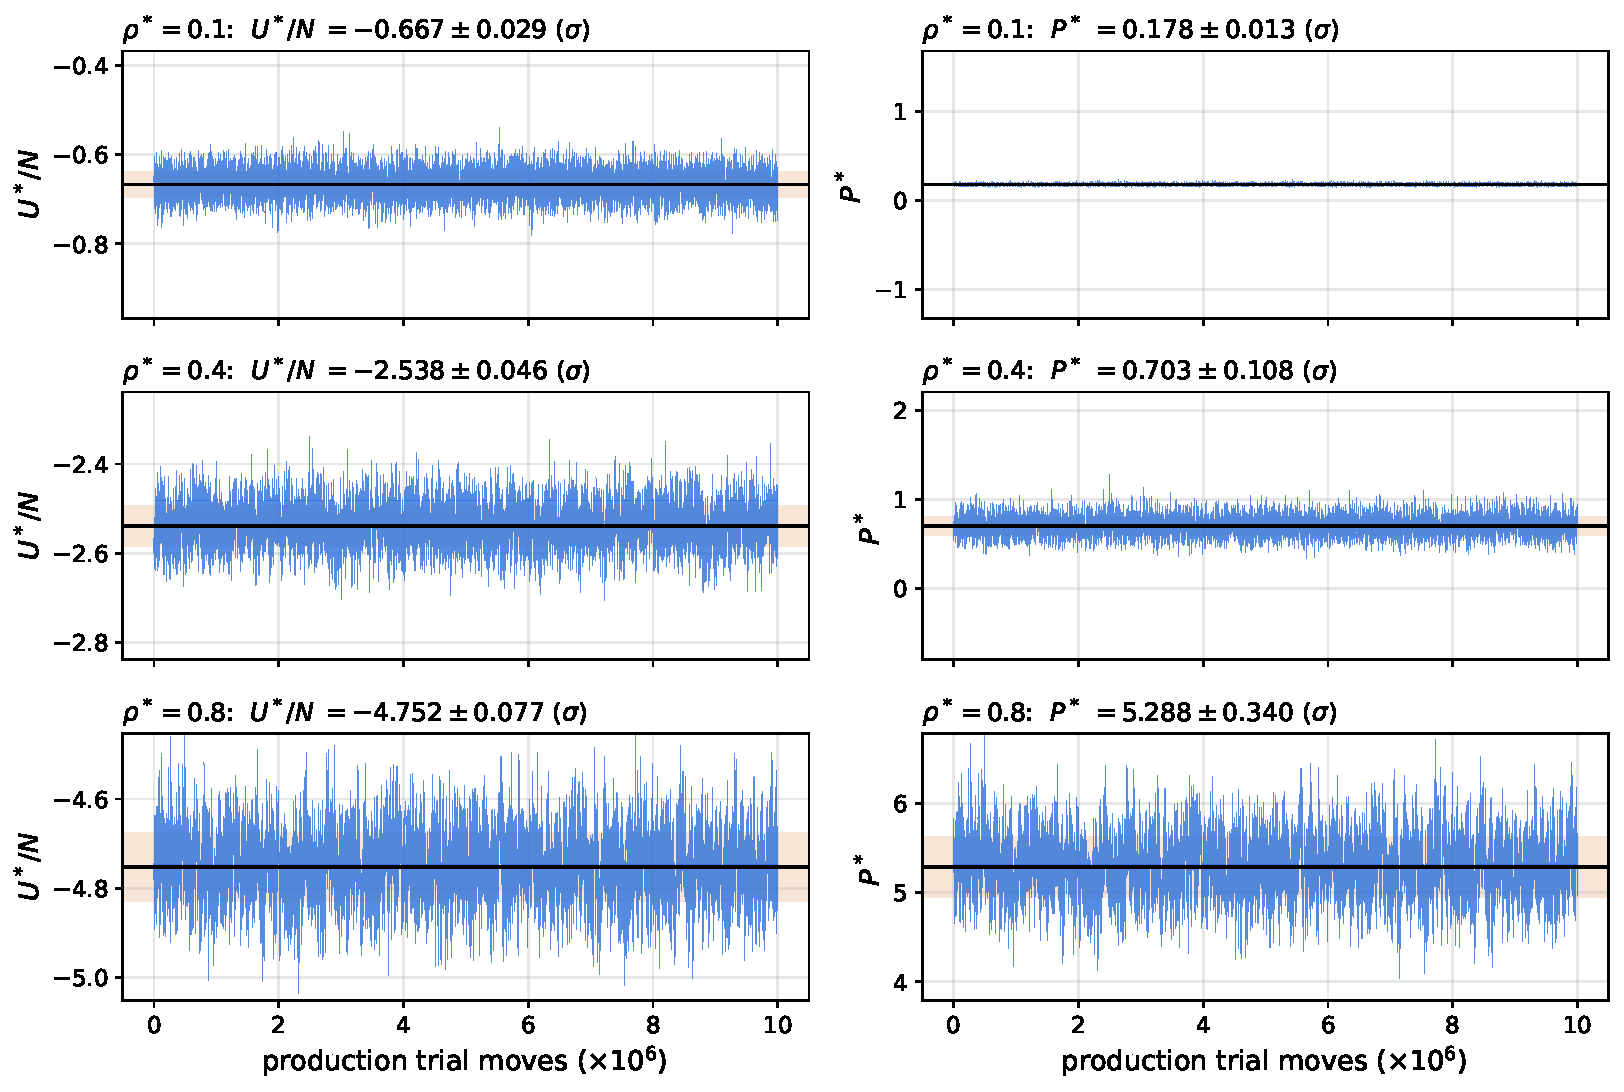
\includegraphics[width=\linewidth]{figures/traces.pdf}
  \caption{Instantaneous energy per atom (left) and pressure (right) during the production run for
  $\rho=0.1$, $0.4$ and $0.8$ at $T=2.0$. All panels have the same $y$ span (0.6 for $U/N$ and 3 for
  $P$), centred on the mean, so the size of the fluctuations can be compared. The black line is the
  mean and the orange band is $\pm\sigma$.}
  \label{fig:traces}
\end{figure}

To compare all the densities at once, \cref{fig:traces_all} puts the eight runs together in one
panel per magnitude. The energy levels are almost equally spaced, since $U/N$ is nearly proportional
to $\rho$, while the pressure levels get further apart at high density. It also shows clearly how the
fluctuations grow with density: at $\rho=0.1$ the pressure is almost a flat line, while at $\rho=0.8$
it spreads over more than one unit.

\begin{figure}[H]
  \centering
  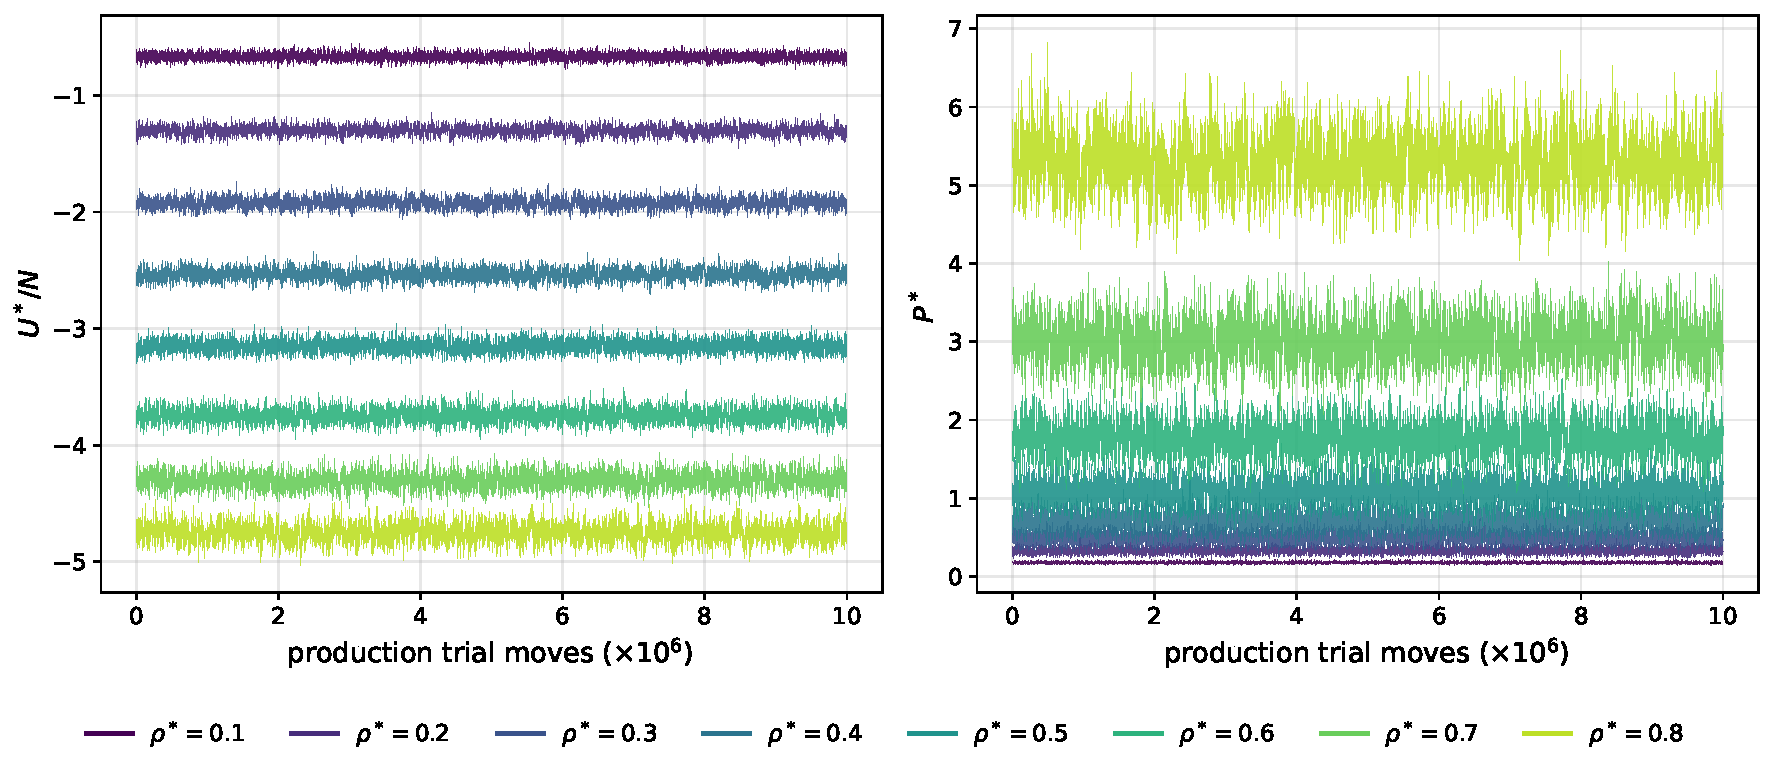
\includegraphics[width=\linewidth]{figures/traces_all.pdf}
  \caption{Instantaneous energy per atom (left) and pressure (right) during the production run for
  all the densities at $T=2.0$.}
  \label{fig:traces_all}
\end{figure}

% ================= EXERCISE 3 =================
\exercise{3}
\statement{Compute the radial distribution function $g(r)$ of the system.}

In \texttt{sample}, every pair distance $r_{ij}<L/2$ is added to a histogram of 200 bins of width
$\delta r = L/400$ (each pair counts twice, once for $i$ and once for $j$). At the end the histogram
is normalised by the number of pairs that an ideal gas would have in the same shell:
\begin{equation}
  g(r_k) = \frac{n_k}{M\,N\,\rho\,\frac{4\pi}{3}\left[(r_k+\delta r)^3 - r_k^3\right]},
  \label{eq:gr}
\end{equation}
where $n_k$ is the accumulated count of bin $k$ and $M$ the number of samples. With this
normalisation $g(r)\to1$ at large $r$. The results are discussed in Exercise 6.

% ================= EXERCISE 4 =================
\exercise{4}
\statement{Perform a series of MC simulations at $T^*=2.0$ and densities from $\rho^*=0.1$ to
$\rho^*=0.8$. Take $n_{\text{cycl}}\sim10^6$--$10^7$. List the technical parameters and the results
($U$, $\sigma_U$, $P$, $\sigma_P$).}

Each density was run in its own folder with $N=500$, $n_{\text{equil}}=10^6$,
$n_{\text{cycl}}=10^7$ production trial moves (i.e.\ $2\times10^4$ moves per atom) and
$n_{\text{samp}}=500$. The technical parameters are listed in \cref{tab:params} and the results in
\cref{tab:results}.

\begin{table}[H]
  \centering
  \caption{Technical parameters of the runs ($T=2.0$, $N=500$, $n_{\text{equil}}=10^6$,
  $n_{\text{cycl}}=10^7$, $n_{\text{samp}}=500$). $\Delta$ is the final maximum displacement.}
  \label{tab:params}
  \begin{tabular}{S[table-format=1.1] S[table-format=2.3] S[table-format=1.3] S[table-format=1.4] S[table-format=1.2]}
    \toprule
    {$\rho$} & {$L$} & {$\Delta$} & {Acceptance} & {$r_c$} \\
    \midrule
    0.1 & 17.100 & 8.550 & 0.5474 & 5.00 \\
    0.2 & 13.572 & 1.435 & 0.4978 & 5.00 \\
    0.3 & 11.856 & 0.875 & 0.4964 & 5.00 \\
    0.4 & 10.772 & 0.629 & 0.4945 & 5.00 \\
    0.5 & 10.000 & 0.471 & 0.5005 & 5.00 \\
    0.6 &  9.410 & 0.373 & 0.4973 & 4.71 \\
    0.7 &  8.939 & 0.299 & 0.4984 & 4.47 \\
    0.8 &  8.550 & 0.240 & 0.5027 & 4.27 \\
    \bottomrule
  \end{tabular}
\end{table}

\begin{table}[H]
  \centering
  \caption{Results at $T=2.0$. $\varepsilon$ is the block error of the mean and $\sigma$ the
  standard deviation of the instantaneous values.}
  \label{tab:results}
  \begin{tabular}{S[table-format=1.1] c S[table-format=1.3] c S[table-format=1.3]}
    \toprule
    {$\rho$} & $U/N$ ($\pm\varepsilon_U$) & {$\sigma_U$} & $P$ ($\pm\varepsilon_P$) & {$\sigma_P$} \\
    \midrule
    0.1 & $-0.6670 \pm 0.0004$ & 0.029 & $0.1776 \pm 0.0001$ & 0.013 \\
    0.2 & $-1.3033 \pm 0.0012$ & 0.038 & $0.3283 \pm 0.0003$ & 0.037 \\
    0.3 & $-1.9232 \pm 0.0015$ & 0.042 & $0.4862 \pm 0.0009$ & 0.068 \\
    0.4 & $-2.5383 \pm 0.0010$ & 0.046 & $0.7030 \pm 0.0022$ & 0.108 \\
    0.5 & $-3.1511 \pm 0.0011$ & 0.049 & $1.0682 \pm 0.0029$ & 0.151 \\
    0.6 & $-3.7473 \pm 0.0011$ & 0.057 & $1.757 \pm 0.004$   & 0.207 \\
    0.7 & $-4.3034 \pm 0.0020$ & 0.065 & $3.007 \pm 0.008$   & 0.266 \\
    0.8 & $-4.7523 \pm 0.0017$ & 0.077 & $5.288 \pm 0.009$   & 0.340 \\
    \bottomrule
  \end{tabular}
\end{table}

It can be seen that the acceptance is \SI{50}{\percent} for all densities except $\rho=0.1$. There the gas is so
dilute that even very big jumps are accepted, and $\Delta$ hits the upper limit we set
($\Delta\le L/2$) with \SI{55}{\percent} acceptance. This is not a problem, it just means
that atoms can jump anywhere in the box. Also, $\Delta$ decreases with density: the denser the fluid, the smaller a displacement has to be
to avoid overlapping with a neighbour. And for $\rho\ge0.6$ the box is smaller than $L=10$, so the cut-off is limited by $L/2$ instead of 5.

Our results agree with the values of Johnson \emph{et al.}\ \cite{johnson} (later on shown and discussed in
\cref{fig:eos,fig:eos_P}).

% ================= EXERCISE 5 =================
\exercise{5}
\statement{Plot the quantities $U^*$ and $P^*$ as a function of $\rho^*$. Up to what density is the
ideal gas law $P=\rho k_BT$ a good approximation?}

\begin{figure}[H]
  \centering
  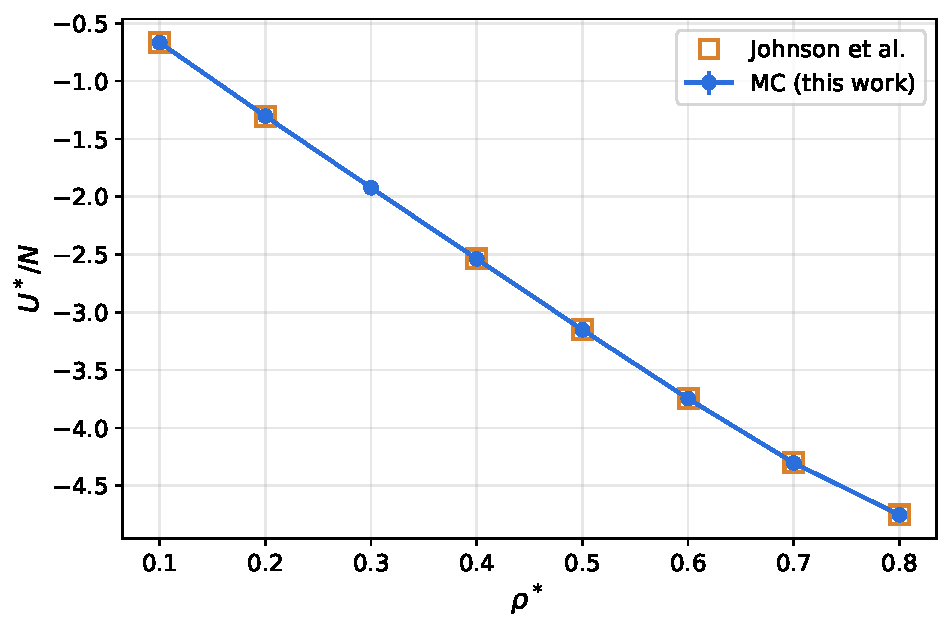
\includegraphics[width=0.75\linewidth]{figures/eos_U.pdf}
  \caption{Energy per atom as a function of density at $T=2.0$. Squares: Johnson \emph{et al.}\
  \cite{johnson}. Error bars (errors of the mean) are smaller than the markers.}
  \label{fig:eos}
\end{figure}

\begin{figure}[H]
  \centering
  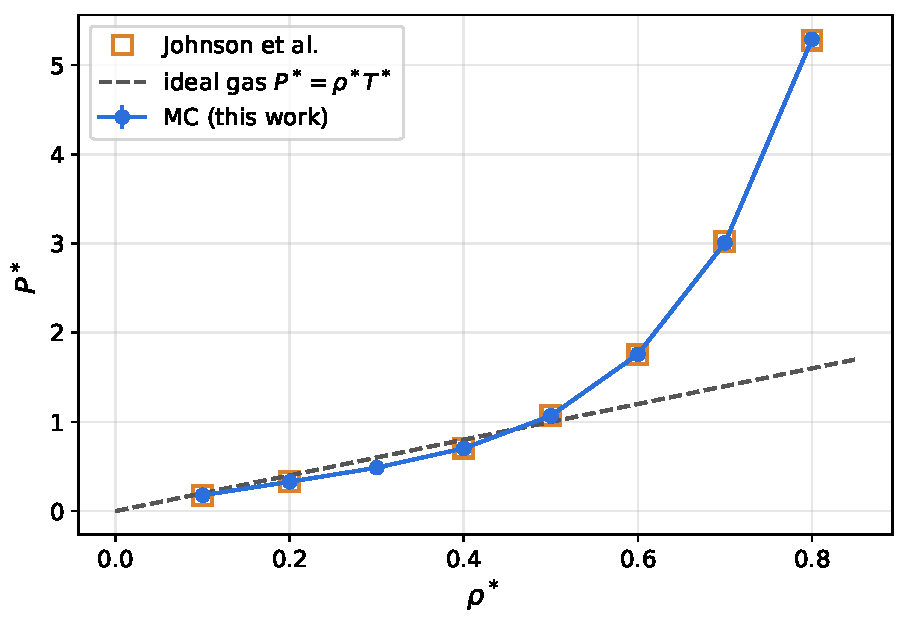
\includegraphics[width=0.75\linewidth]{figures/eos_P.pdf}
  \caption{Pressure as a function of density at $T=2.0$. Squares: Johnson \emph{et al.}\
  \cite{johnson}. Dashed line: ideal gas. Error bars are smaller than the markers.}
  \label{fig:eos_P}
\end{figure}

\Cref{fig:eos} shows that $U/N$ decreases almost linearly with $\rho$: at low density each atom has
on average $\sim\rho$ neighbours inside the attractive well, so the energy is roughly proportional
to $\rho$. \Cref{fig:eos_P} shows that the pressure grows slowly at low density and then much
faster than the ideal gas line. In both cases our points lie on top of the reference values of Johnson \emph{et al.}\ \cite{johnson}.

To answer the question it is easier to look at the compressibility factor $Z=P/(\rho T)$
(\cref{fig:eos_Z}), which is exactly 1 for an ideal gas.

\begin{figure}[H]
  \centering
  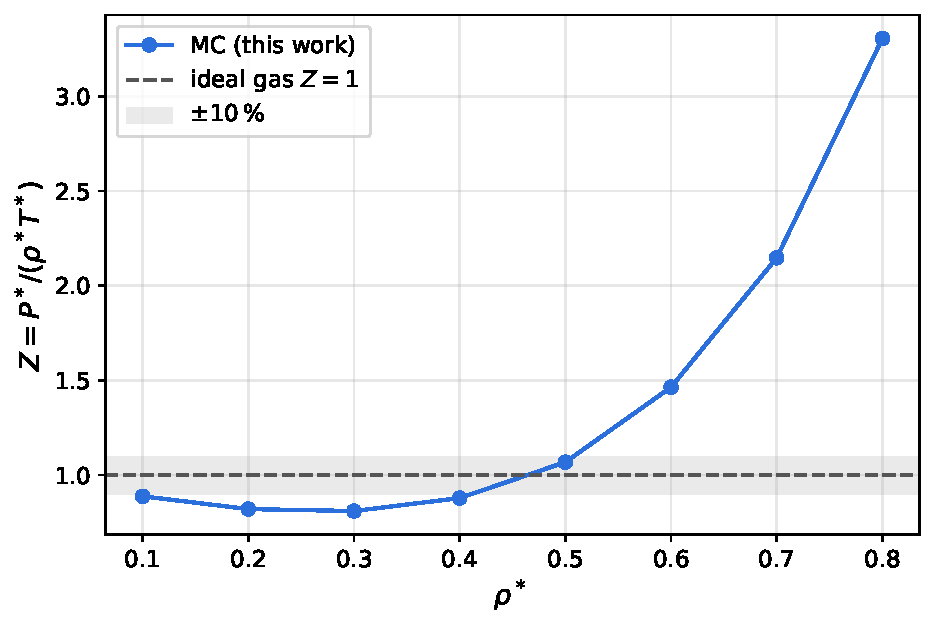
\includegraphics[width=0.75\linewidth]{figures/eos_Z.pdf}
  \caption{Compressibility factor $Z=P/(\rho T)$ as a function of density at $T=2.0$. The dashed
  line is the ideal gas ($Z=1$) and the grey band marks a $\pm\SI{10}{\percent}$ deviation.}
  \label{fig:eos_Z}
\end{figure}

The zoom in \cref{fig:eos_zoom} and the values of $Z$ give:

\begin{table}[H]
  \centering
  \caption{Compressibility factor $Z=P/(\rho T)$ from the simulations.}
  \label{tab:Z}
  \begin{tabular}{l *{8}{S[table-format=1.2]}}
    \toprule
    $\rho$ & 0.1 & 0.2 & 0.3 & 0.4 & 0.5 & 0.6 & 0.7 & 0.8 \\
    \midrule
    $Z$    & 0.89 & 0.82 & 0.81 & 0.88 & 1.07 & 1.46 & 2.15 & 3.31 \\
    \bottomrule
  \end{tabular}
\end{table}

\begin{figure}[H]
  \centering
  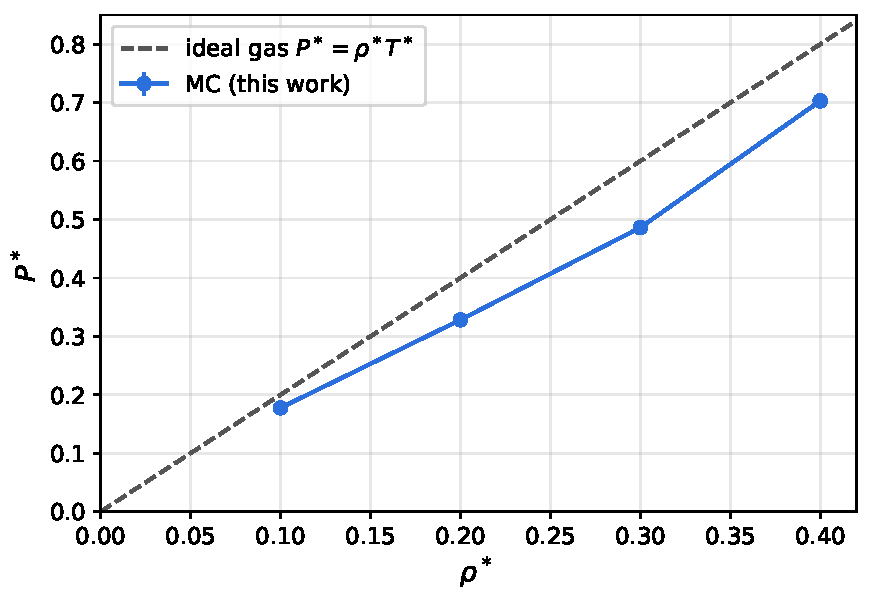
\includegraphics[width=0.6\linewidth]{figures/eos_zoom.pdf}
  \caption{Zoom of the equation of state at low density compared with the ideal gas law.}
  \label{fig:eos_zoom}
\end{figure}

Already at $\rho=0.1$ the pressure is slightly below the ideal gas value, because the
attractive part of the potential pulls the atoms together and reduces the pressure. Between
$\rho=0.2$ and $0.4$ the deviation is close to \SI{20}{\percent}. Around $\rho\approx0.46$ we get
$Z\approx1$ again, but this is just a coincidence where the attractive and repulsive parts cancel
($U/N\approx-3$ is far from the ideal value 0). Above $\rho=0.5$ the repulsive core dominates and
$P$ grows much faster than $\rho T$ ($Z=3.3$ at $\rho=0.8$). So the ideal gas law is only a good
approximation up to $\rho\approx0.1$ as molecules interactions are much weaker; for higher densities it cannot be used.

% ================= EXERCISE 6 =================
\exercise{6}
\statement{Plot the functions $g(r)$ obtained for the different densities.}

\begin{figure}[H]
  \centering
  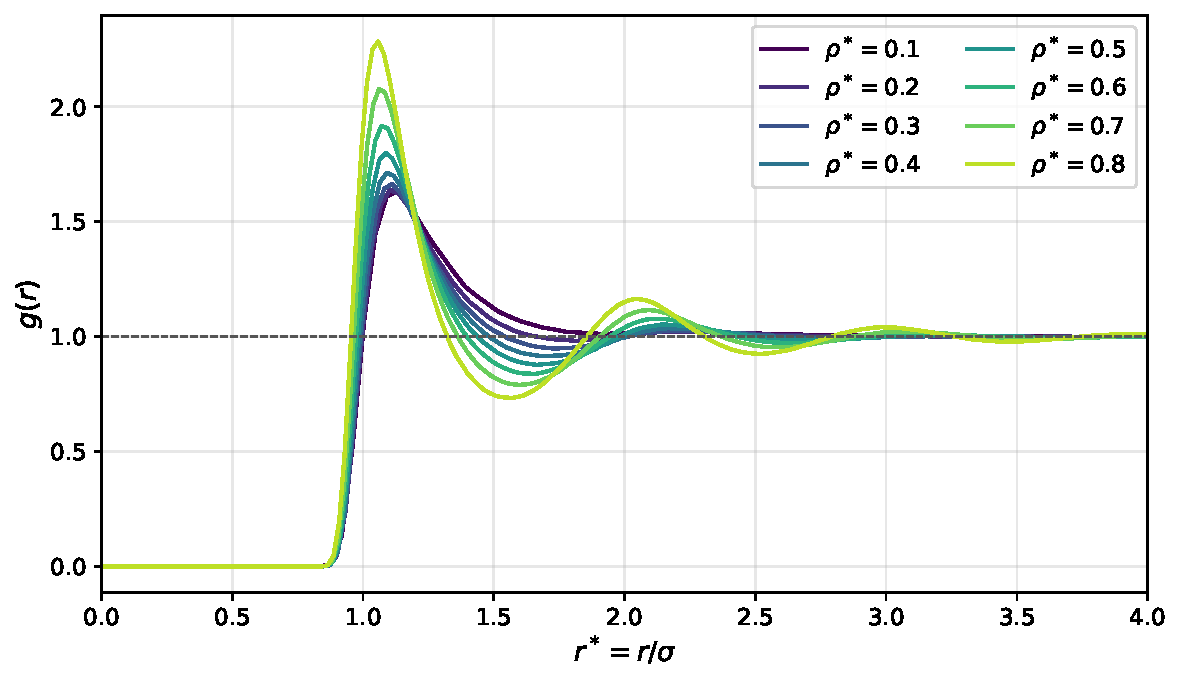
\includegraphics[width=0.85\linewidth]{figures/rdf_all.pdf}
  \caption{Radial distribution function at $T=2.0$ for all the densities. The dashed line is $g=1$.}
  \label{fig:rdf}
\end{figure}

\begin{figure}[H]
  \centering
  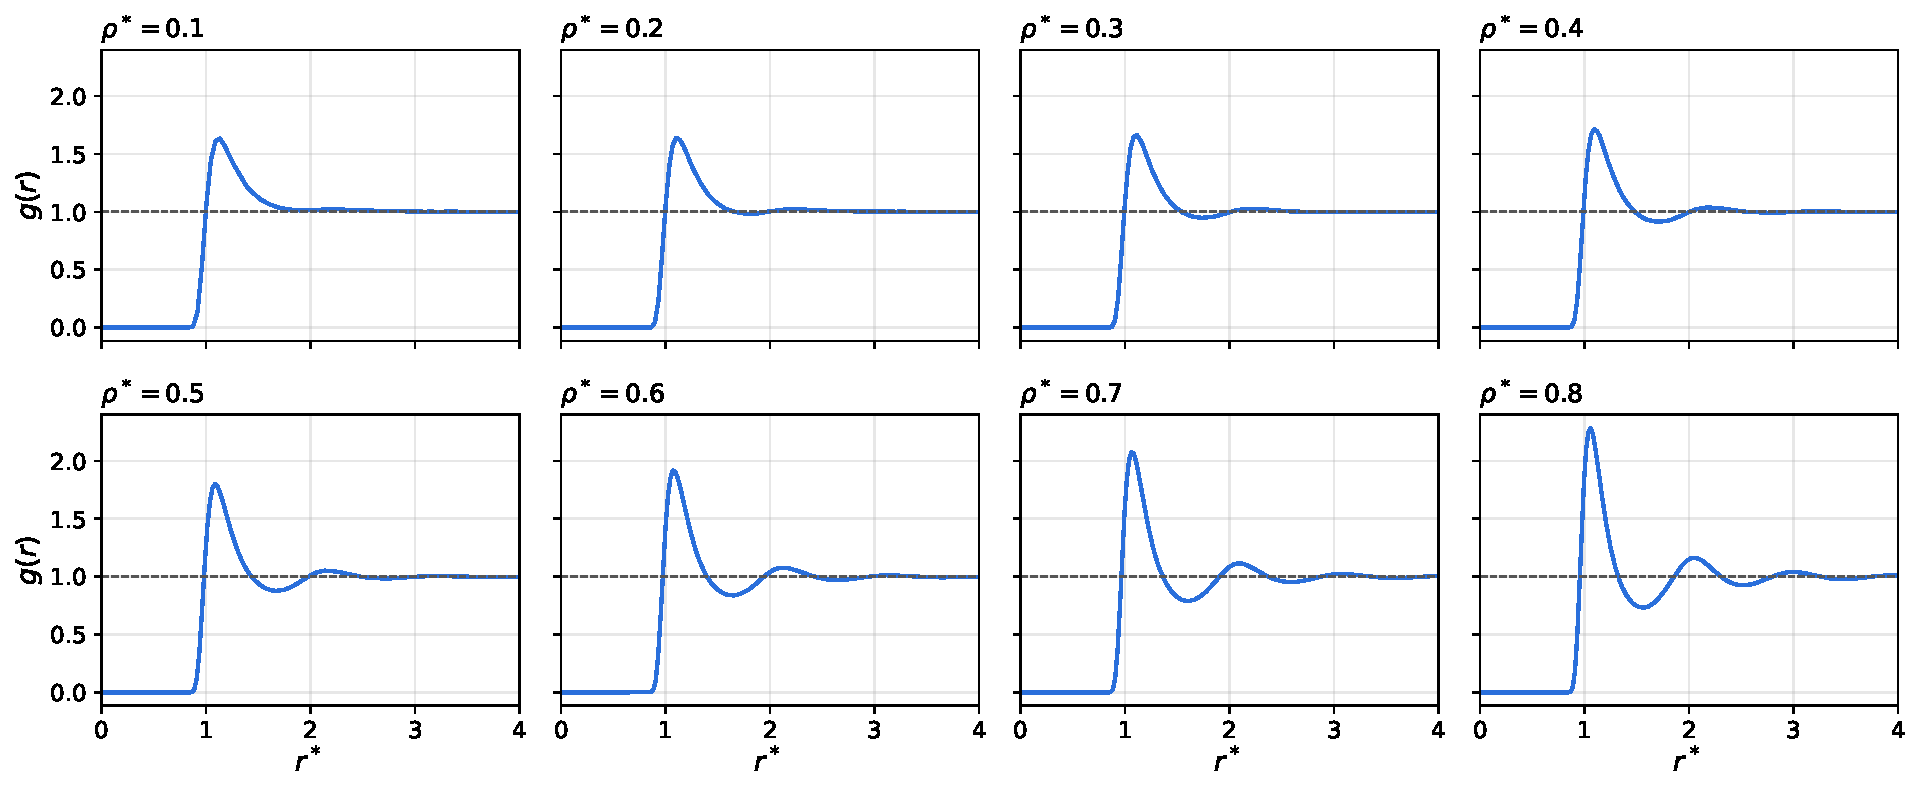
\includegraphics[width=\linewidth]{figures/rdf_grid.pdf}
  \caption{The same $g(r)$ as in \cref{fig:rdf}, one panel per density, to see each shape clearly.}
  \label{fig:rdf_grid}
\end{figure}

All the curves (\cref{fig:rdf,fig:rdf_grid}) have the same general features:
\begin{itemize}
  \item $g(r)=0$ for $r\lesssim0.9$: two atoms cannot get closer than about $\sigma$ because of
        the Lennard-Jones repulsion.
  \item A first peak near the minimum of the potential around $r\approx 1$. The peak moves slightly inwards by increasing
        the density because at high density the neighbours are pushed closer together.
  \item At low density, after the first peak $g(r)$ goes to 1, but as $\rho$ increases a second (around $r\approx2$) and
        even a third shell appear.
  \item In all cases $g(r)\to1$ at large $r$, so the normalisation of \cref{eq:gr} is correct.
\end{itemize}

% ================= EXERCISE 7 =================
\exercise{7}
\statement{The energy and pressure can also be obtained by numerical integration of the RDF. Make
the numerical integrations, and compare the results with the direct calculation of these properties
carried out in Step 4.}

Using $g(r)$ the sums over pairs in \cref{eq:UP} become integrals:
\begin{equation}
  \frac{U}{N} = 2\pi\rho\int_0^{r_c} u(r)\,g(r)\,r^2\,dr + \frac{U_{\text{tail}}}{N},
  \qquad
  P = \rho T - \frac{2\pi\rho^2}{3}\int_0^{r_c} \frac{du}{dr}\,g(r)\,r^3\,dr + P_{\text{tail}},
  \label{eq:integrals}
\end{equation}
with $du/dr = -48r^{-13}+24r^{-7}$. We integrate up to the same $r_c$ as in the simulation and add
the same tail corrections, so that both routes compute exactly the same quantity. The integrals are
done with the trapezoidal rule over the bin centres of $g(r)$ (script in \hyperref[app:python]{Appendix B}).

\begin{table}[H]
  \centering
  \caption{Comparison between the direct averages (Exercise 4) and the integration of $g(r)$.}
  \label{tab:ex7}
  \begin{tabular}{S[table-format=1.1]
                  S[table-format=-1.4] S[table-format=-1.4] S[table-format=1.2]
                  S[table-format=1.4] S[table-format=1.4] S[table-format=1.2]}
    \toprule
    {$\rho$} & {$U/N$ direct} & {$U/N$ from $g(r)$} & {Diff.\ (\si{\percent})}
             & {$P$ direct} & {$P$ from $g(r)$} & {Diff.\ (\si{\percent})} \\
    \midrule
    0.1 & -0.6670 & -0.6635 & 0.52 & 0.1776 & 0.1795 & 1.06 \\
    0.2 & -1.3033 & -1.2987 & 0.36 & 0.3283 & 0.3332 & 1.50 \\
    0.3 & -1.9232 & -1.9181 & 0.27 & 0.4862 & 0.4945 & 1.71 \\
    0.4 & -2.5383 & -2.5322 & 0.24 & 0.7030 & 0.7162 & 1.87 \\
    0.5 & -3.1511 & -3.1438 & 0.23 & 1.0682 & 1.0873 & 1.78 \\
    0.6 & -3.7473 & -3.7385 & 0.24 & 1.7572 & 1.7843 & 1.55 \\
    0.7 & -4.3034 & -4.2925 & 0.25 & 3.0066 & 3.0449 & 1.27 \\
    0.8 & -4.7523 & -4.7391 & 0.28 & 5.2883 & 5.3404 & 0.99 \\
    \bottomrule
  \end{tabular}
\end{table}

\begin{figure}[H]
  \centering
  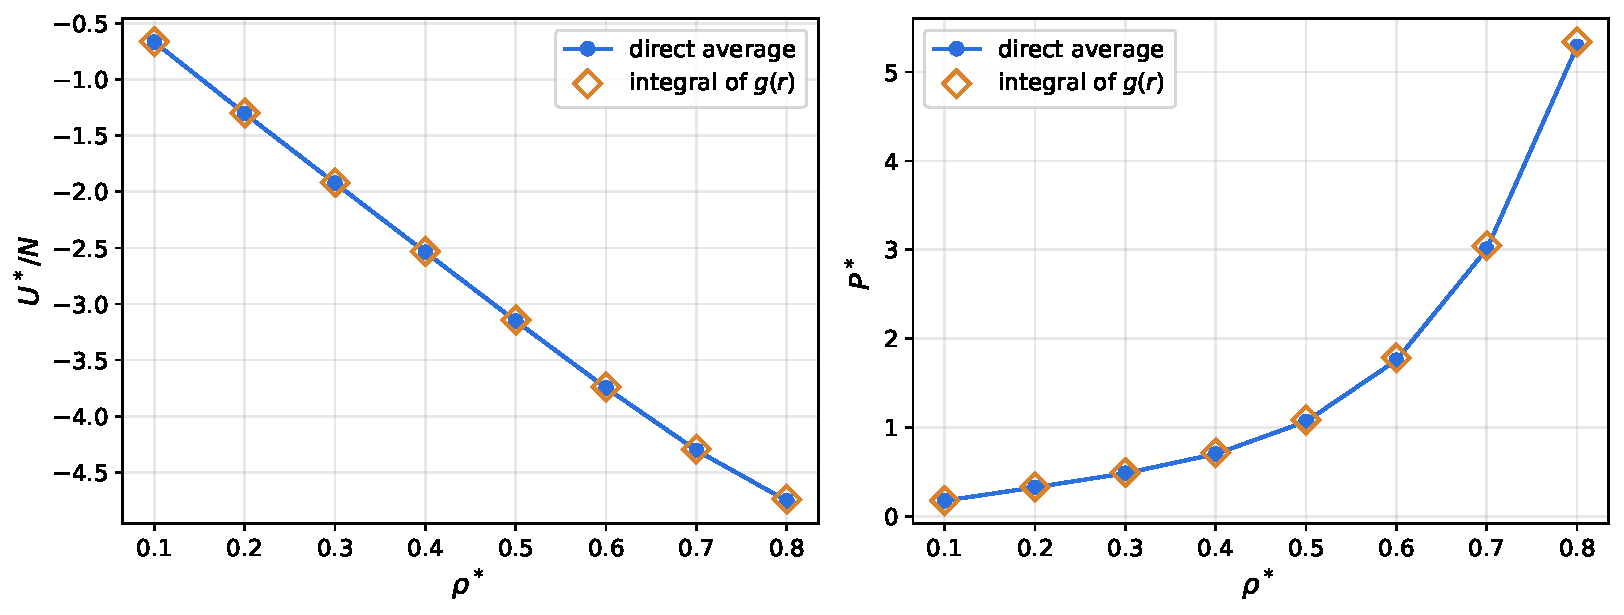
\includegraphics[width=0.95\linewidth]{figures/rdf_integration.pdf}
  \caption{Energy per atom (left) and pressure (right) obtained directly in the simulation and by
  integrating $g(r)$ with \cref{eq:integrals}.}
  \label{fig:ex7}
\end{figure}

Both methods agree well (\cref{tab:ex7,fig:ex7}): the differences are below \SI{0.5}{\percent} for
the energy and below \SI{2}{\percent} for the pressure, and on the scale of the plot the points are
on top of each other. In any case, the direct calculation during the simulation is the more accurate one.

% ================= REFERENCES =================
\begin{thebibliography}{9}
\bibitem{johnson} J.~K.~Johnson, J.~A.~Zollweg and K.~E.~Gubbins,
  ``The Lennard-Jones equation of state revisited'', \emph{Mol.\ Phys.}\ \textbf{78}, 591 (1993).
\end{thebibliography}

% ================= APPENDIX =================
\newpage
\appendix
\section*{A.\quad Code for the MC simulation (\texttt{mcnvt.f90})}
\phantomsection\label{app:code}
\addcontentsline{toc}{section}{A. Code for the MC simulation}
\lstinputlisting[style=fortran]{code/mcnvt.f90}

Input file \texttt{mc-lj.data} used for $\rho=0.1$ (only the density line changes between runs):
\lstinputlisting[style=terminal]{code/mc-lj.data}

\section*{B.\quad Code for the figures and the $g(r)$ integration (\texttt{make\_figures.py})}
\phantomsection\label{app:python}
\addcontentsline{toc}{section}{B. Code for the figures}
\lstinputlisting[style=python]{make_figures.py}

\end{document}
